\appendix
\chapter{Statistics} \label{ch:appendix_statistic}
\section{Temporal statistics} \label{sec:all_stats}
%%% ALL LOCAL STATISTICS FOR VARIABLES 
%% TEMPERATURE
\begin{figure}[ht]
    \centering
    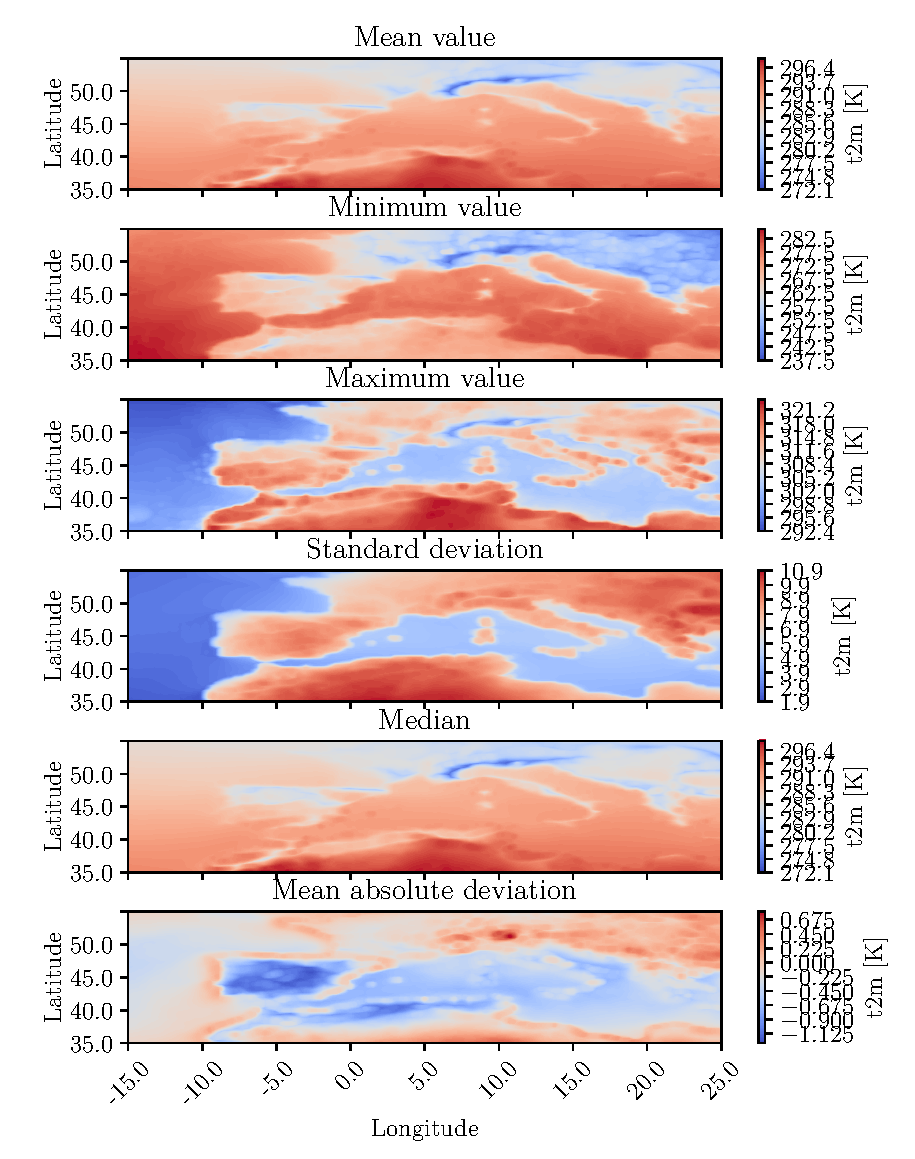
\includegraphics{python_figs/all_stat_variable_t2m.pdf}
    \caption{Contour plot showing the local (pixel) statistics for temperature.}
    \label{fig:all_stats_t2m}
\end{figure}

%% SURFACE PRESSURE 
\begin{figure}[ht]
    \centering
    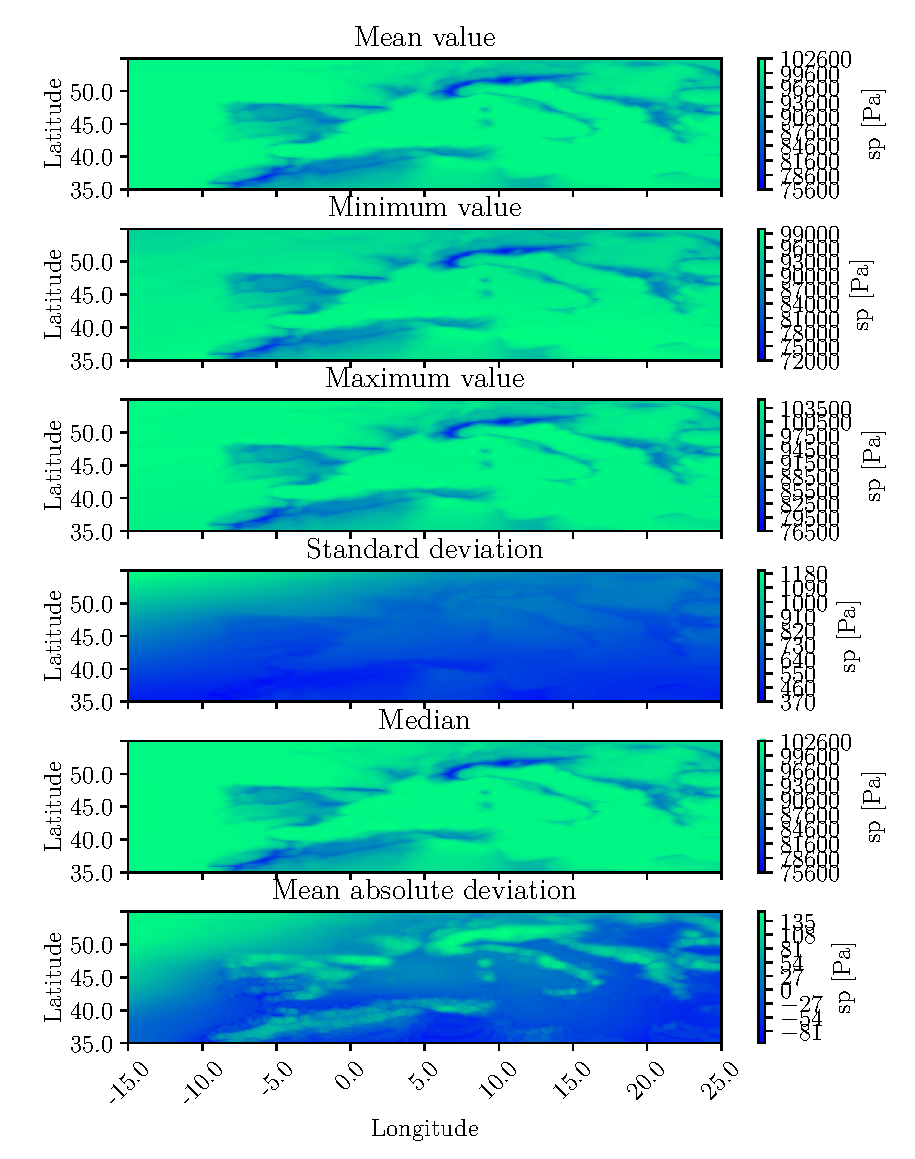
\includegraphics{python_figs/all_stat_variable_sp.pdf}
    \caption{Contour plot showing the local (pixel) statistics for surface pressure.}
    \label{fig:all_stats_sp}
\end{figure}

%% RELATIVE HUMIDITY 
\begin{figure}[ht]
    \centering
    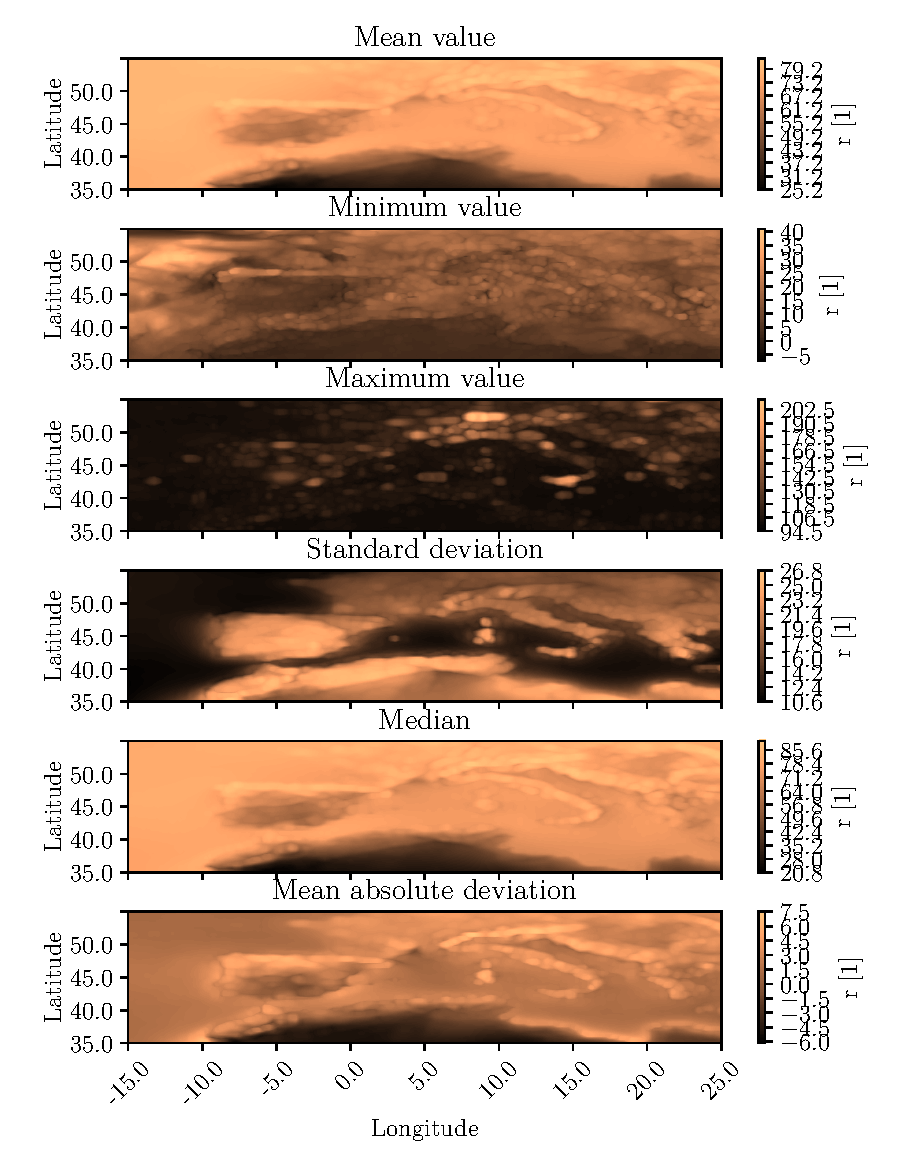
\includegraphics{python_figs/all_stat_variable_r.pdf}
    \caption{Contour plot showing the local (pixel) statistics for relative humidity.}
    \label{fig:all_stats_r}
\end{figure}

%% SPECIFIC HUMIDITY 
\begin{figure}[ht]
    \centering
    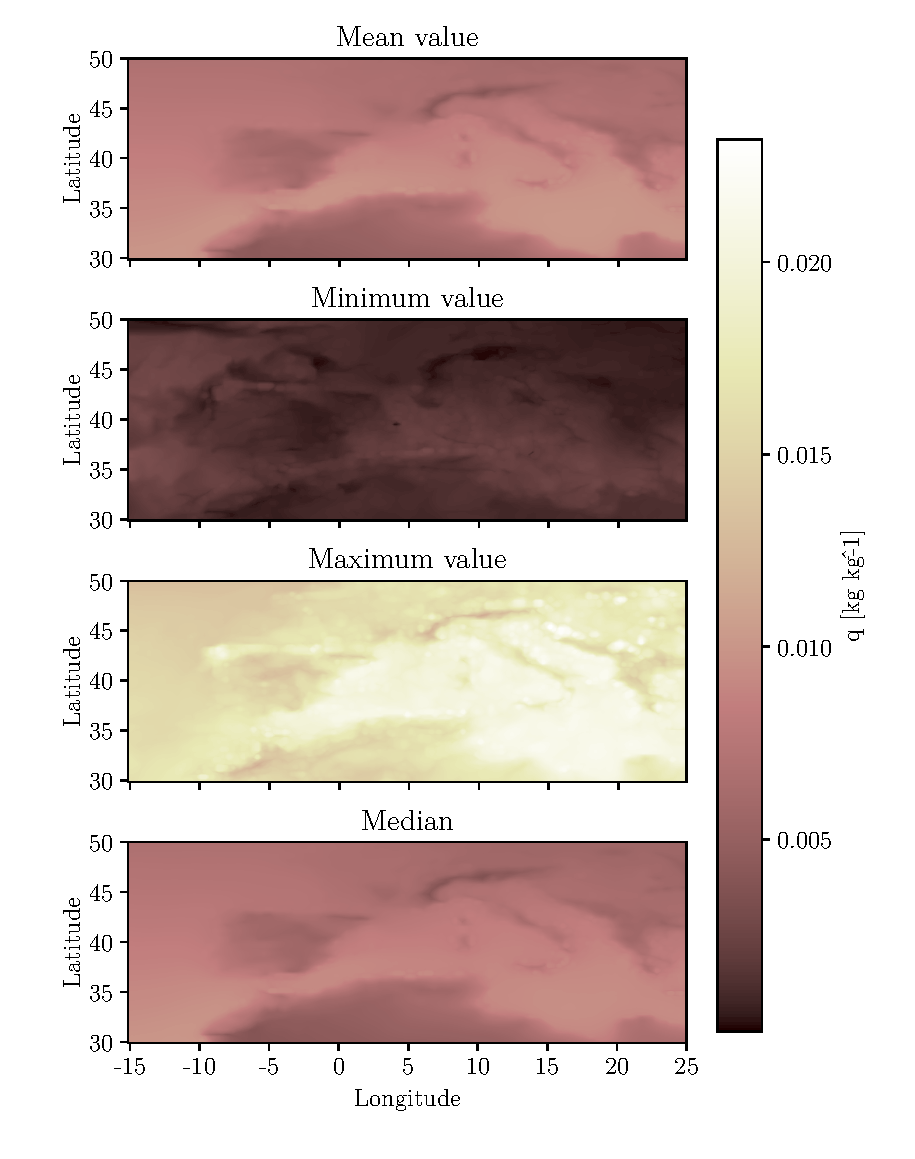
\includegraphics{python_figs/all_stat_variable_q.pdf}
    \caption{Contour plot showing the local (pixel) statistics for specific humidity.}
    \label{fig:all_stats_q}
\end{figure}

\section{Temporal statistics deviations} \label{sec:all_stats_deviation}
\begin{figure}
    \centering
    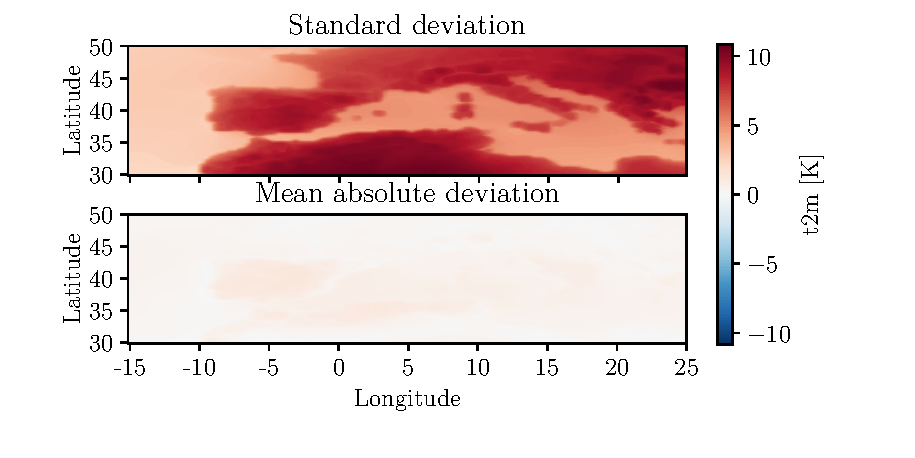
\includegraphics{python_figs/DEVIATION_all_stat_variable_t2m.pdf}
    \caption{Deviations in two meter temperature, $t_2m$.}
    \label{fig:deviation_t2m}
\end{figure}

\begin{figure}
    \centering
    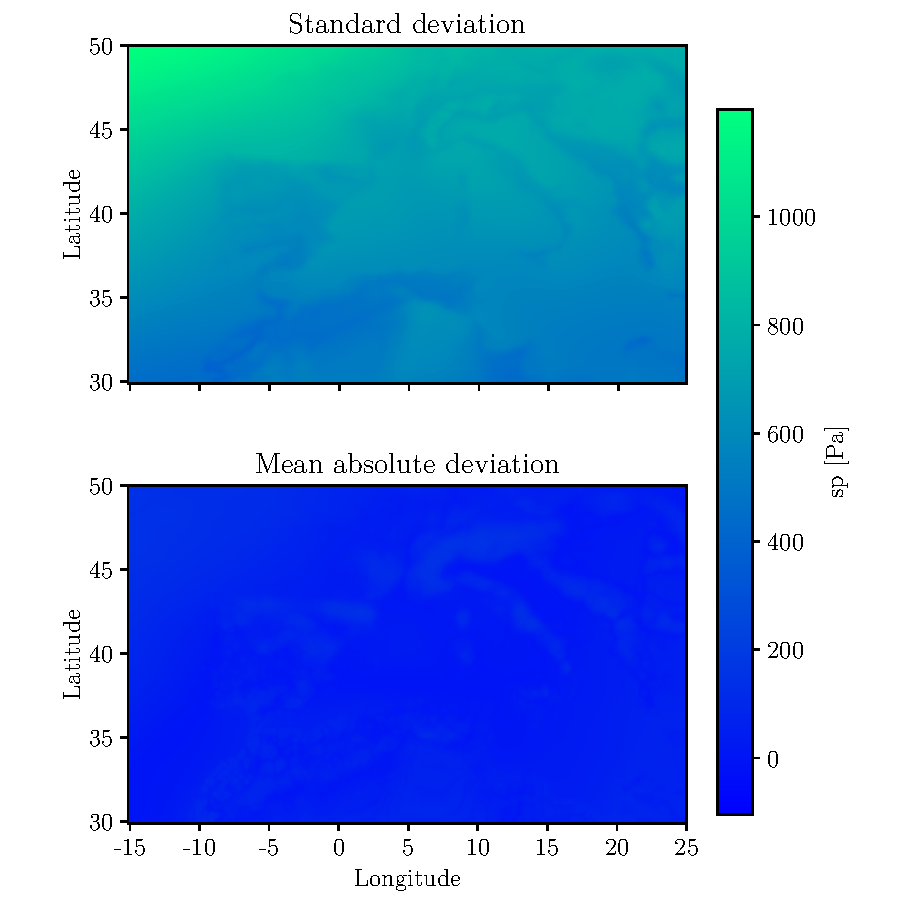
\includegraphics{python_figs/DEVIATION_all_stat_variable_sp.pdf}
    \caption{Deviations in surface pressure, sp.}
    \label{fig:deviation_sp}
\end{figure}

\begin{figure}
    \centering
    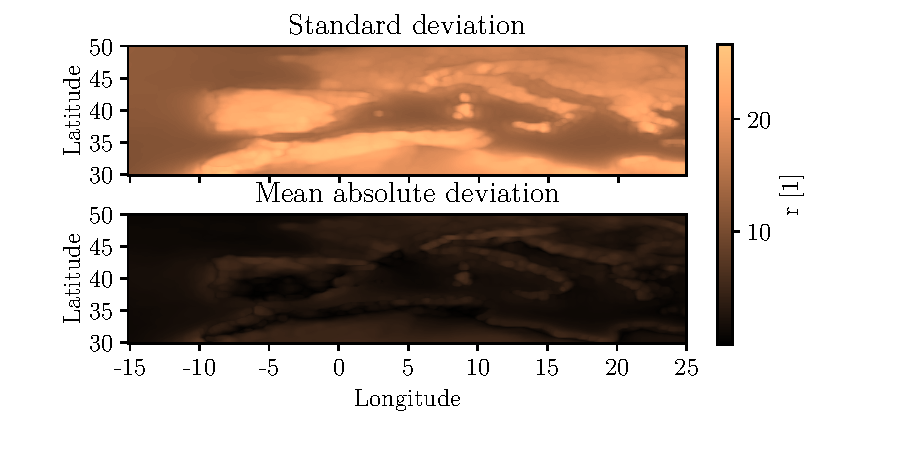
\includegraphics{python_figs/DEVIATION_all_stat_variable_r.pdf}
    \caption{Deviations in relative humidity, r.}
    \label{fig:deviation_r}
\end{figure}


\begin{figure}
    \centering
    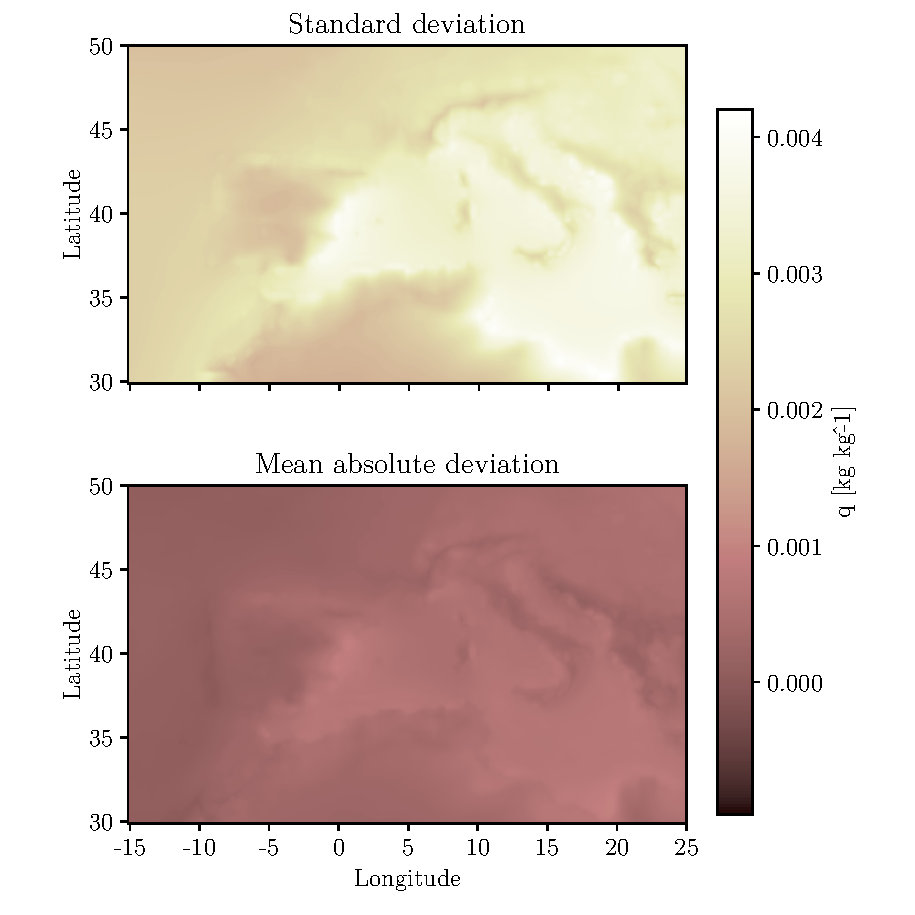
\includegraphics{python_figs/DEVIATION_all_stat_variable_q.pdf}
    \caption{Deviations in specific humidity, q.}
    \label{fig:deviation_q}
\end{figure}


\cleardoublepage

\chapter{Seasonal effects} \label{app:seasonal_plots}
\begin{figure}[ht]
    \centering
    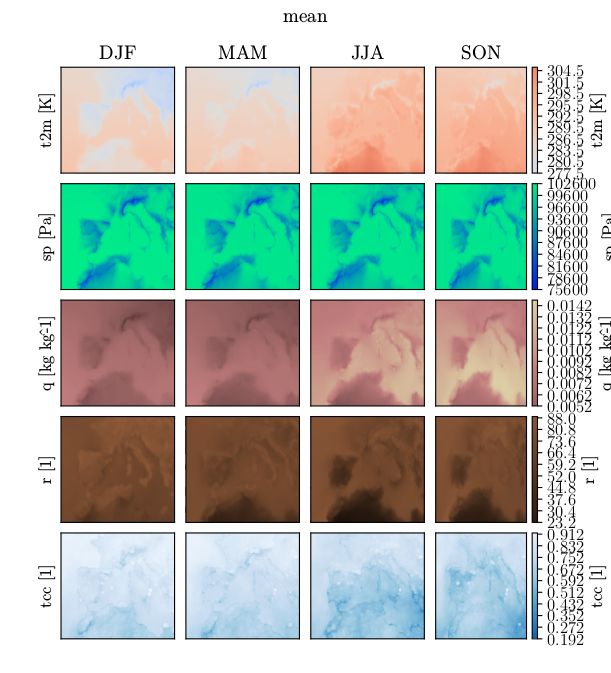
\includegraphics{python_figs/seasonal_mean_all_variables.png}
    \caption{Seasonal mean}
    \label{fig:seasonal_mean}
\end{figure}

\begin{figure}[ht]
    \centering
    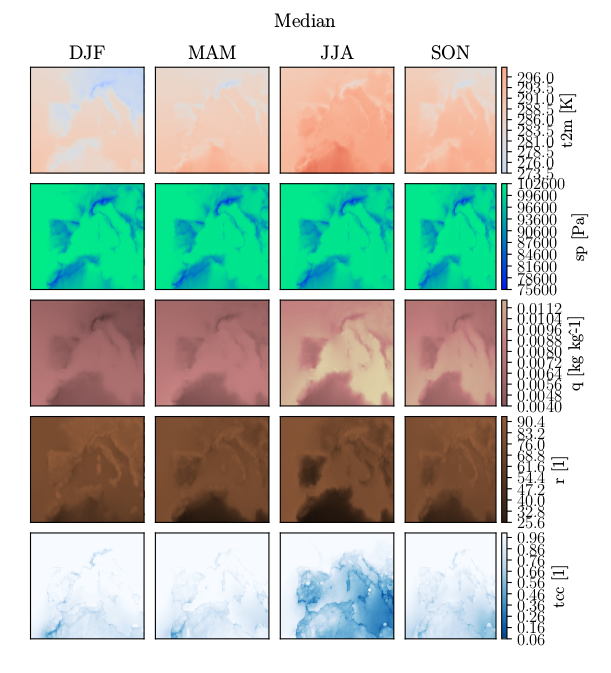
\includegraphics{python_figs/seasonal_median_all_variables.png}
    \caption{Seasonal median}
    \label{fig:seasonal_median}
\end{figure}


\chapter{Timelapse of \acrlong{cfc} } \label{app:timelapse}

\begin{figure}[ht]
    \centering
    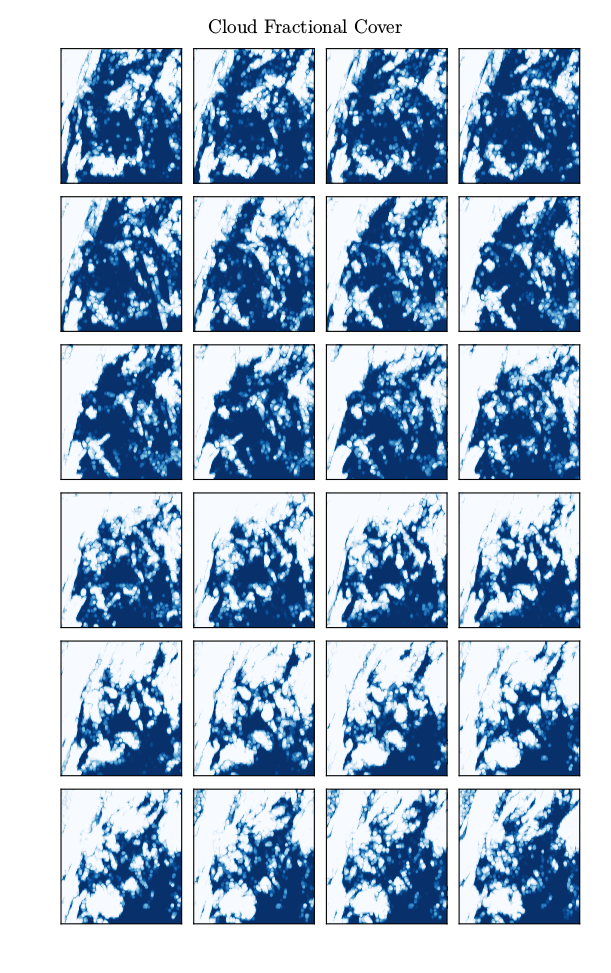
\includegraphics[scale=0.70]{python_figs/timelapse_cloud_cover_24hrs_from_2010-07-01.png}
    \caption{Time lapse photo illustrating changes in cloud cover occuring within 24 hours from first of July 2010.}
    \label{fig:time_lapse}
\end{figure}


\chapter{First week of every month in 2012} \label{app:first_week}
%\addcontentsline{toc}{chapter}{Appendix D: Study 2012}

\begin{figure}[ht]
    \centering
    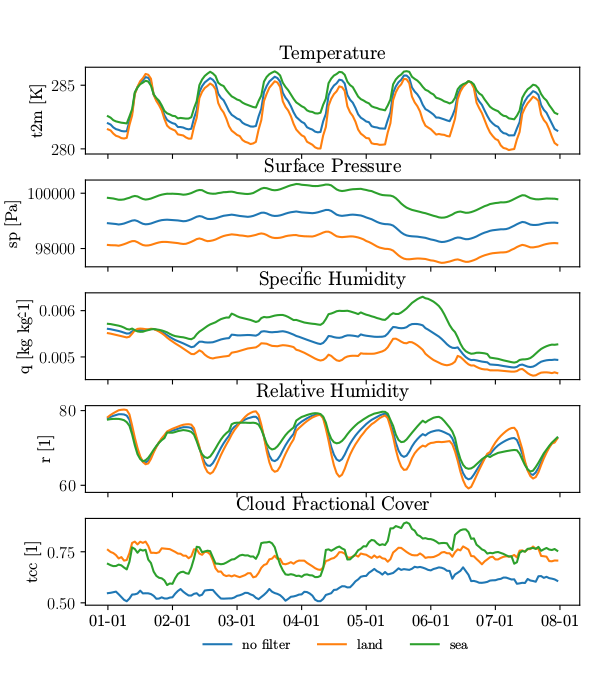
\includegraphics{python_figs/spatially_averaged_one_week_from_2012-01-01.png}
    \caption{Signal January 2012.}
    \label{fig:jan12}
\end{figure}

\begin{figure}[ht]
    \centering
    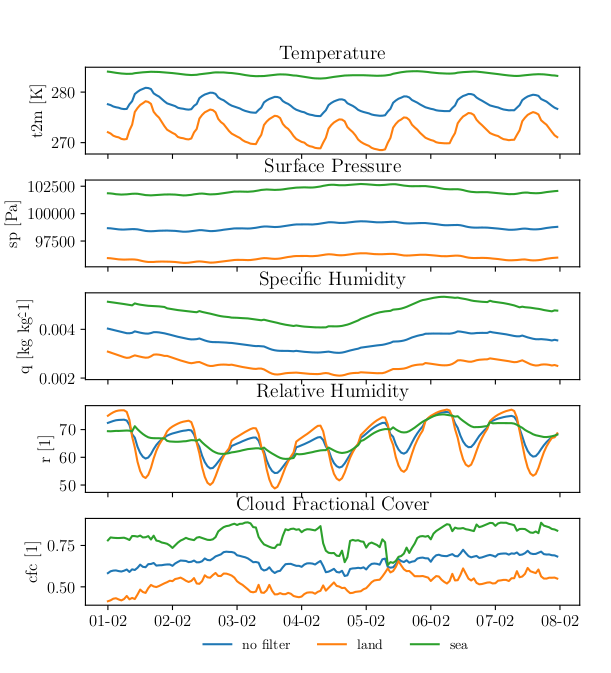
\includegraphics{python_figs/spatially_averaged_one_week_from_2012-02-01.png}
    \caption{Signal February 2012.}
    \label{fig:feb12}
\end{figure}

\begin{figure}[ht]
    \centering
    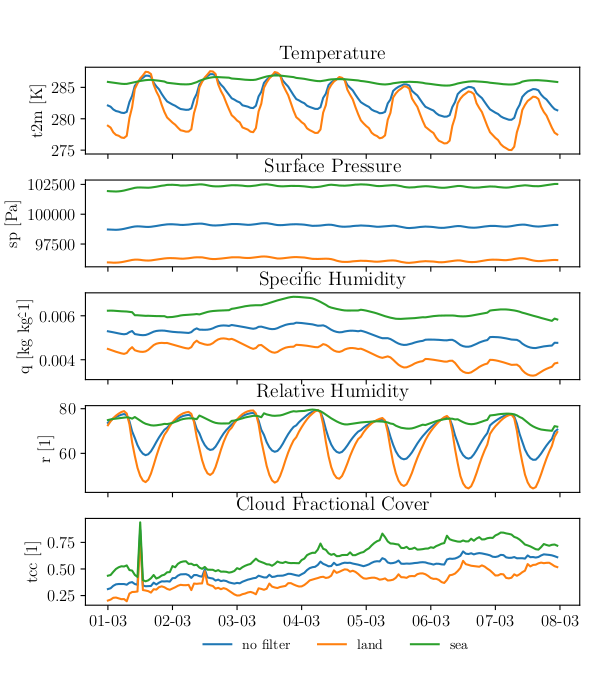
\includegraphics{python_figs/spatially_averaged_one_week_from_2012-03-01.png}
    \caption{Signal March 2012.}
    \label{fig:mar12}
\end{figure}

\begin{figure}[ht]
    \centering
    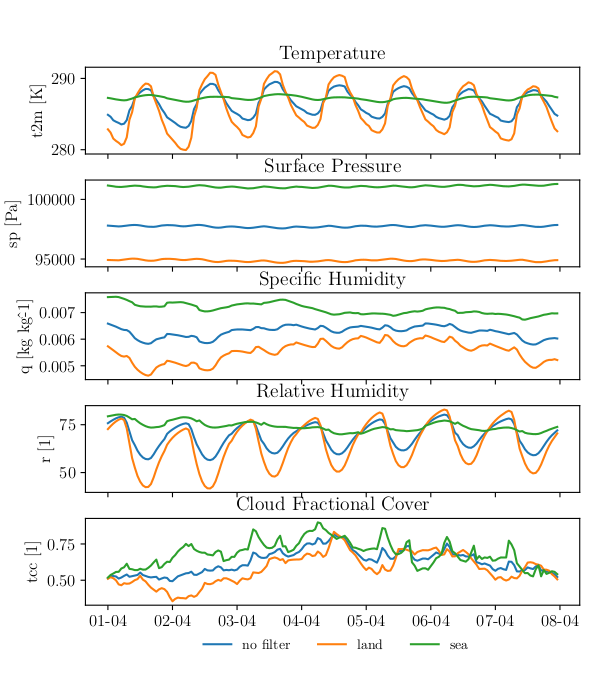
\includegraphics{python_figs/spatially_averaged_one_week_from_2012-04-01.png}
    \caption{Signal April 2012.}
    \label{fig:april12}
\end{figure}

\begin{figure}[ht]
    \centering
    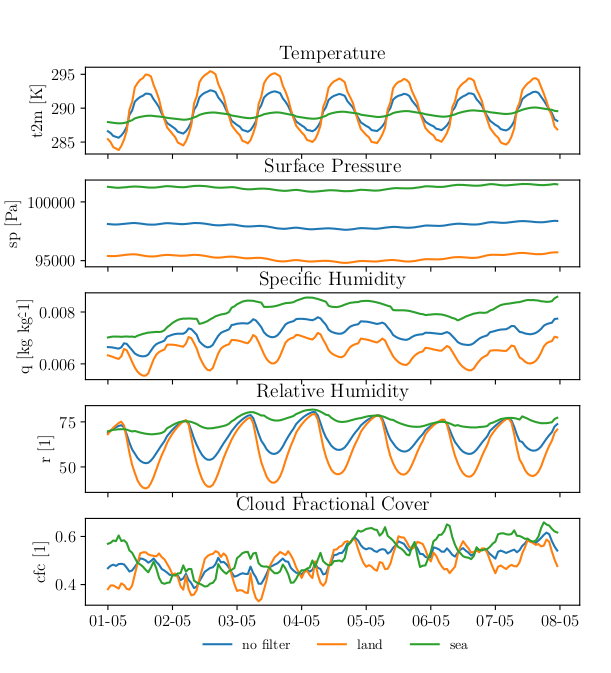
\includegraphics{python_figs/spatially_averaged_one_week_from_2012-05-01.png}
    \caption{Signal May 2012.}
    \label{fig:may12}
\end{figure}


\begin{figure}[ht]
    \centering
    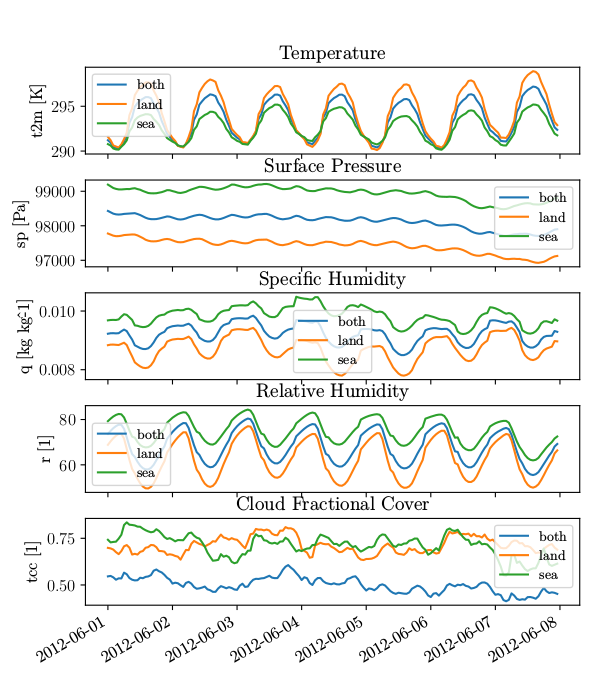
\includegraphics{python_figs/spatially_averaged_one_week_from_2012-06-01.png}
    \caption{Signal June 2012.}
    \label{fig:jun12}
\end{figure}

\begin{figure}[ht]
    \centering
    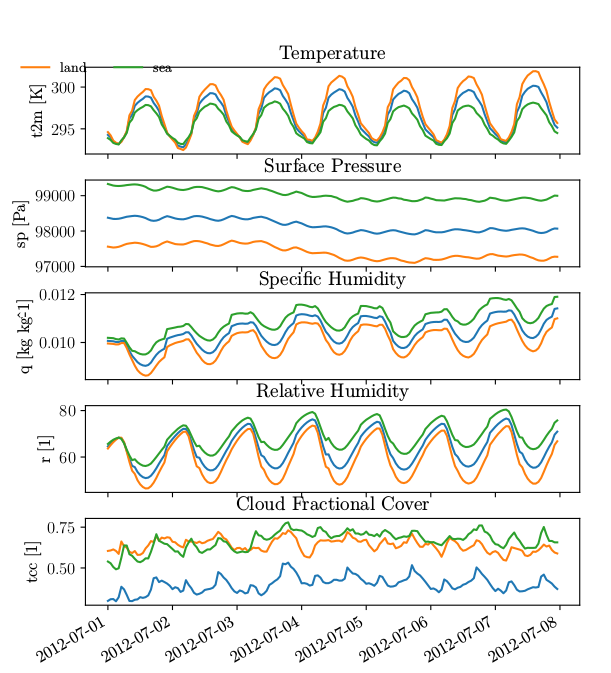
\includegraphics{python_figs/spatially_averaged_one_week_from_2012-07-01.png}
    \caption{Signal July 2012.}
    \label{fig:jul12}
\end{figure}


\begin{figure}[ht]
    \centering
    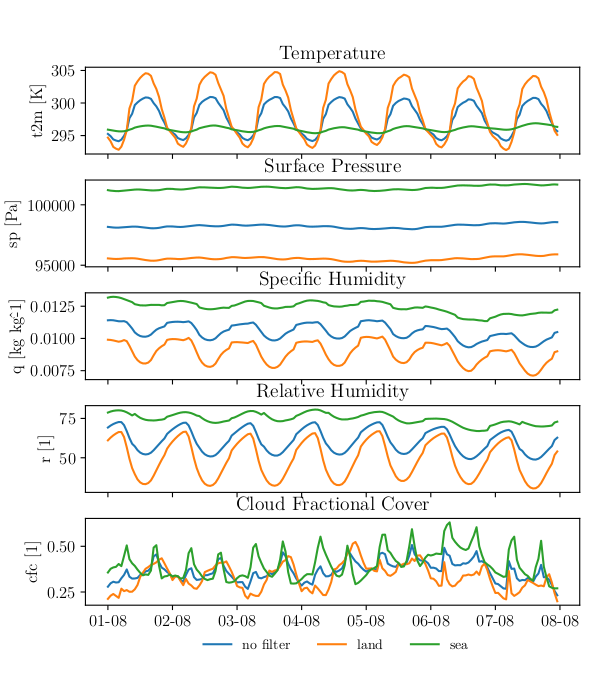
\includegraphics{python_figs/spatially_averaged_one_week_from_2012-08-01.png}
    \caption{Signal August 2012.}
    \label{fig:aug12}
\end{figure}

% September is in the text

\begin{figure}[ht]
    \centering
    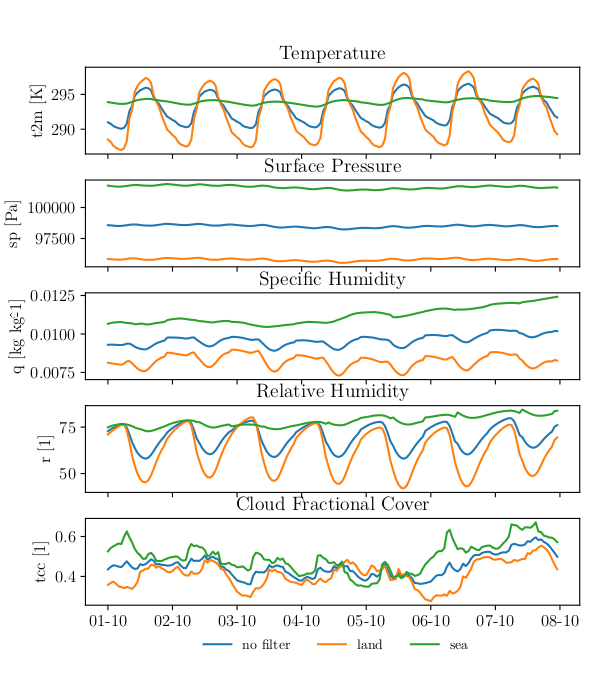
\includegraphics{python_figs/spatially_averaged_one_week_from_2012-10-01.png}
    \caption{Signal October 2012.}
    \label{fig:oct12}
\end{figure}


\begin{figure}[ht]
    \centering
    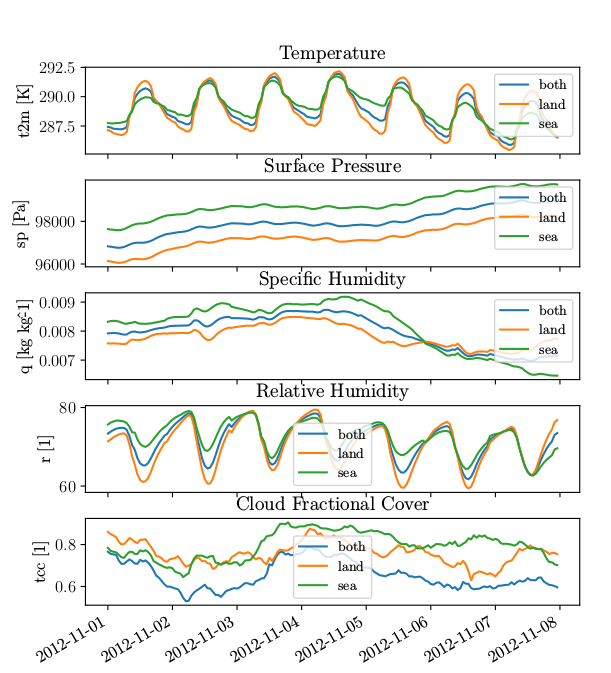
\includegraphics{python_figs/spatially_averaged_one_week_from_2012-11-01.png}
    \caption{Signal November 2012.}
    \label{fig:nov12}
\end{figure}

\begin{figure}[ht]
    \centering
    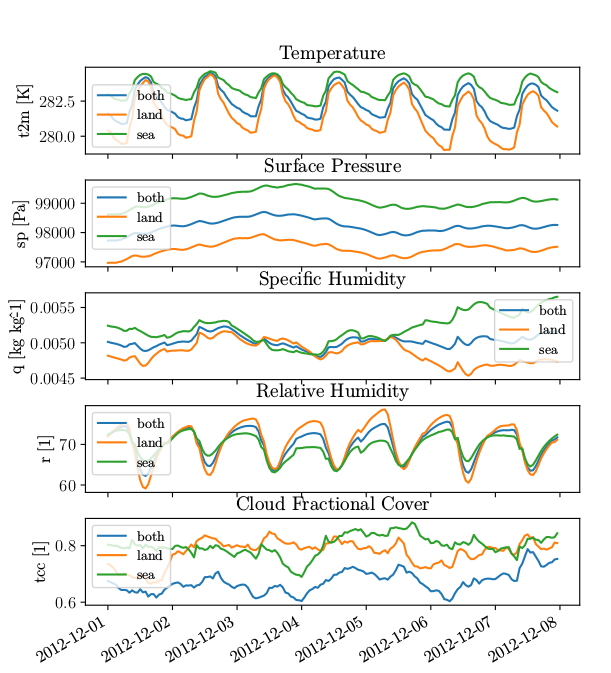
\includegraphics{python_figs/spatially_averaged_one_week_from_2012-12-01.png}
    \caption{Signal December 2012.}
    \label{fig:dec12}
\end{figure}

\cleardoublepage



\chapter{Performance of other models} 
Currently it show the plots that could be generated to show the performance for other model. The plots below is generated based on dummy data. 

\section{Listing of non-trainable architectures} \label{app:list_non_trainable_architectures}
As a reference to future studies below is a listing of non-trainable architectures.
\begin{enumerate}
    \item $ConvLSTM-B_{10}-SL_{24}-128-3\times3$
    \item $ConvLSTM-B_{10}-SL_{24}-128-3\times3-32-3\times3$
    \item $ConvLSTM-B_{10}-SL_{24}-64-3\times3-64-3\times3$
    \item $ConvLSTM-B_{5}-SL_{24}-256-3\times3-256-3\times3$
    \item $ConvLSTM-B_{5}-SL_{6}-256-3\times3-256-3\times3$
\end{enumerate}

%\textbf{List of models trained to slow, will be finished in 6 days. \textbf{Double check config.}}
%\begin{enumerate}
%    \item $ConvLSTM-B_{5}-SL_{6}-256-3\times3$
%    \item $ConvLSTM-B_{5}-SL_{6}-256-1\times1$
%\end{enumerate}

\section{Prediction sequence ConvLSTM 1x1 filter}
\begin{figure}
    \centering
    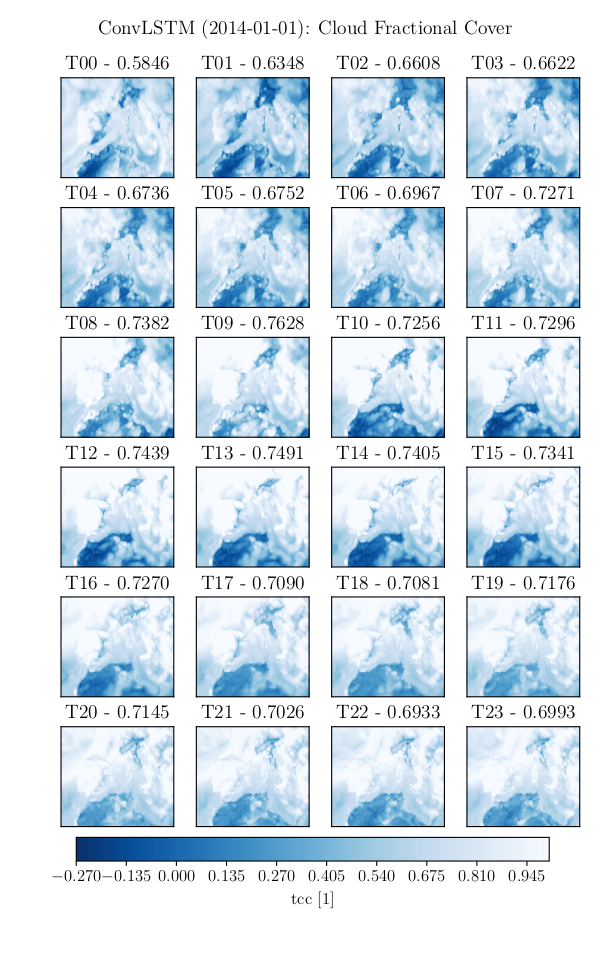
\includegraphics{python_figs/timelapse_convlstm_1x1_24hrs_from_2014-01-01.png}
    \caption{Timelapse prediction, same configuration as best model except for the $1\times1$ filter.}
    \label{fig:timelapse_1x1}
\end{figure}

\section{Performance of AR-models}

\begin{figure}
    \centering
    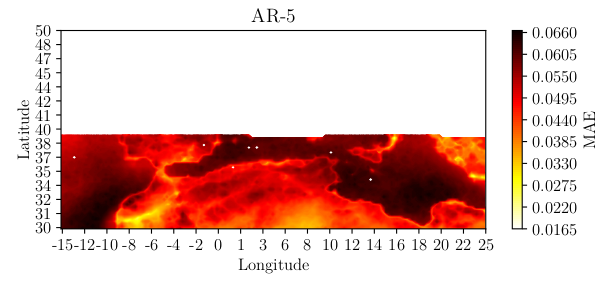
\includegraphics{python_figs/mea_best_ar_model_tcc_AR_L1_in_folder_AR-5.png}
    \caption{Caption}
    \label{fig:my_label}
\end{figure}

\begin{figure}
    \centering
    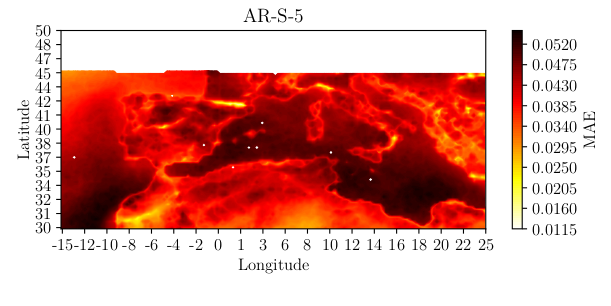
\includegraphics{python_figs/mea_best_ar_model_tcc_AR_L1_in_folder_AR-S-5.png}
    \caption{Caption}
    \label{fig:my_label}
\end{figure}

\begin{figure}
    \centering
    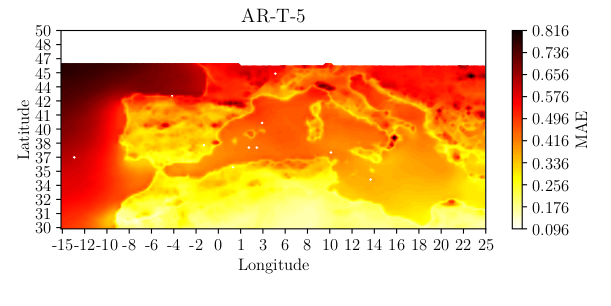
\includegraphics{python_figs/mea_best_ar_model_tcc_AR_L1_in_folder_AR-T-5.png}
    \caption{Caption}
    \label{fig:my_label}
\end{figure}

\cleardoublepage

\chapter{All four parts of example prediction} \label{app:pred_sequence}
\textbf{OBS this duplicates the first one}

\begin{figure}
    \centering
    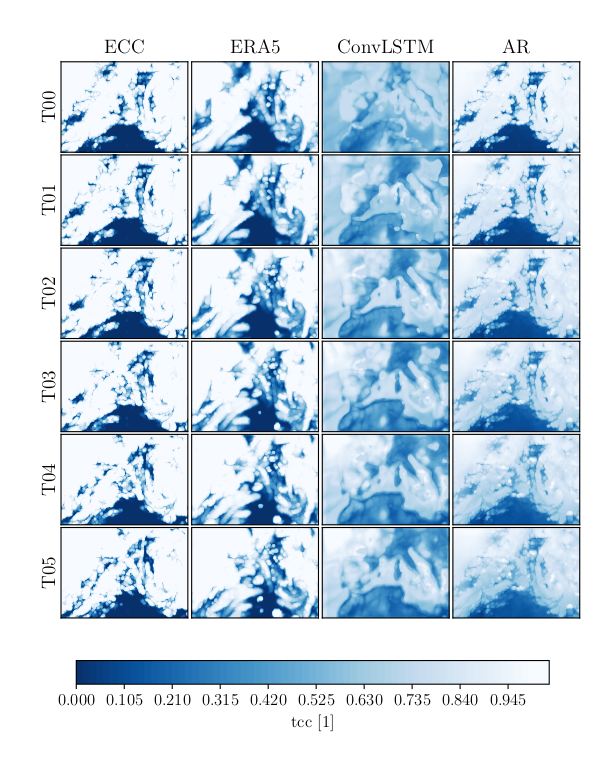
\includegraphics[scale=0.9]{python_figs/comparting_seq_part_1_of4.png}
    \caption{Part 1/4 of the predicted 24 hours sequence }
    \label{fig:part1/4}
\end{figure}

\begin{figure}
    \centering
    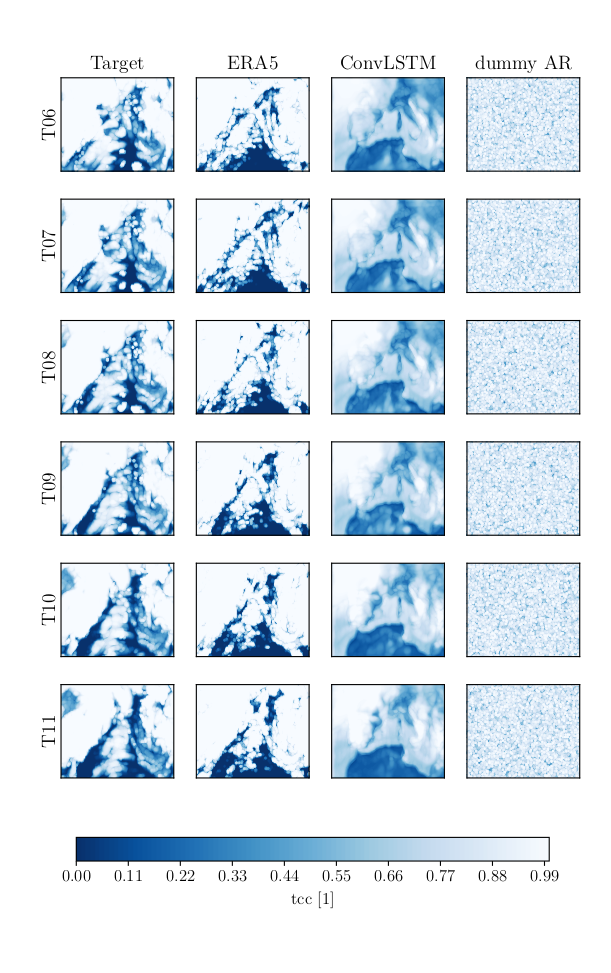
\includegraphics{python_figs/comparting_seq_part_2_of4.png}
    \caption{Part 2/4 of the predicted 24 hours sequence }
    \label{fig:part2/4}
\end{figure}

\begin{figure}
    \centering
    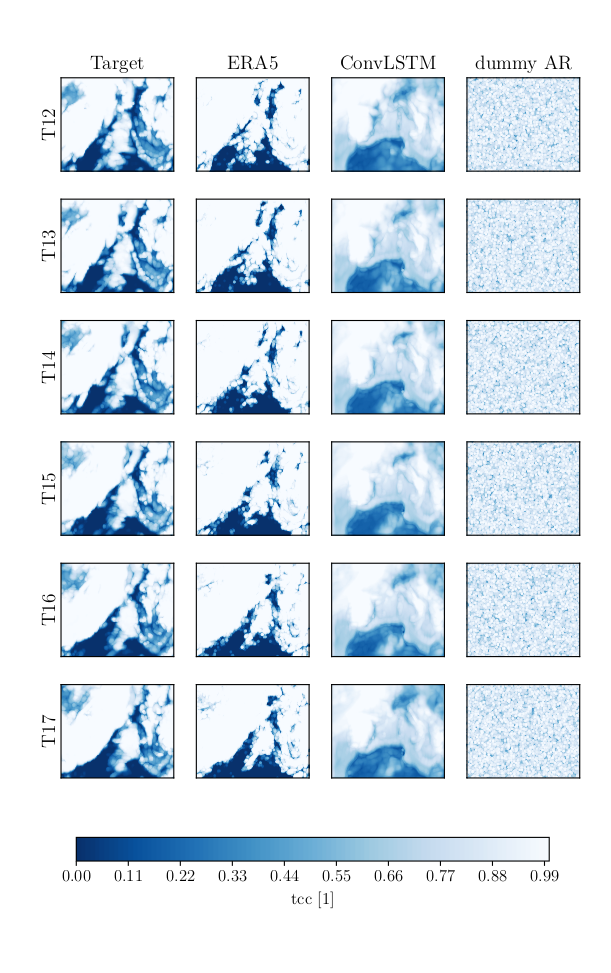
\includegraphics{python_figs/comparting_seq_part_3_of4.png}
    \caption{Part 3/4 of the predicted 24 hours sequence }
    \label{fig:part3/4}
\end{figure}

\begin{figure}
    \centering
    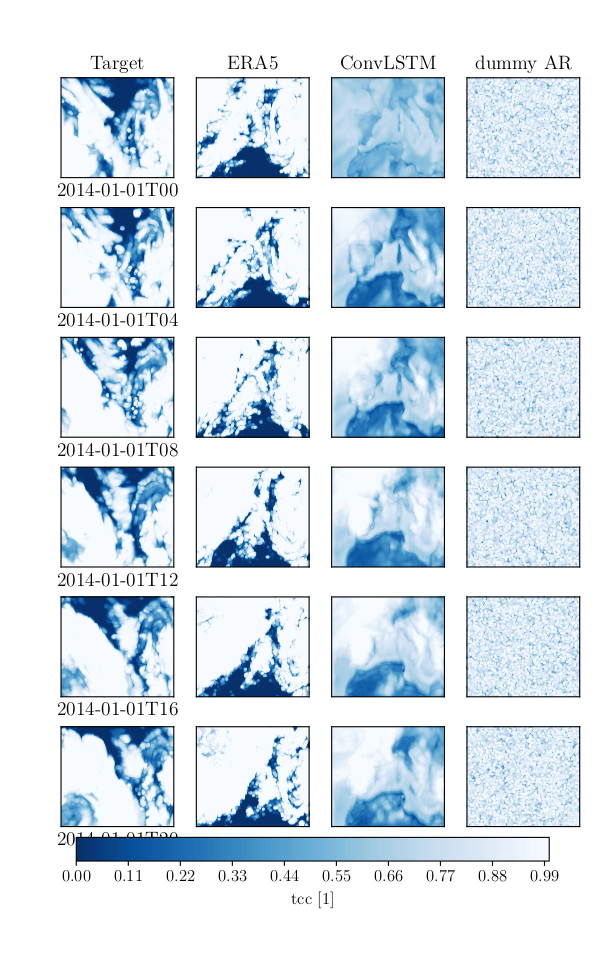
\includegraphics{python_figs/comparting_seq_part_4_of4.png}
    \caption{Part 4/4 of the predicted 24 hours sequence }
    \label{fig:part4/4}
\end{figure}

\cleardoublepage

%%%%%%%%%%%%%%%%%%%%%%%%%%%%%%%%%%%%% signal artefact should be redefined if used 
\chapter{Miscellaneous} \label{app:misc}

\begin{figure}
    \centering
    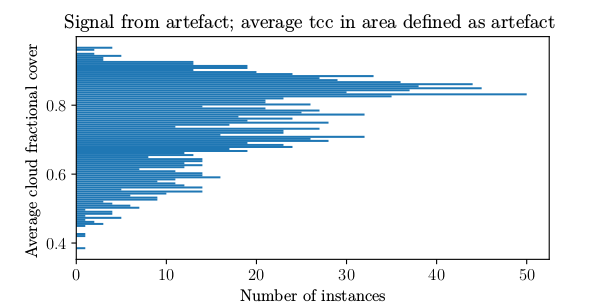
\includegraphics{python_figs/signal_artefact.png}
    \caption{Occurrence of artefact, keep in mind that is not made any effort to distinguish this from when the entire area has cloud cover, this could be done by the ratio of artefact signal to land or something else. }
    \label{fig:signal_artefact}
\end{figure}
